\documentclass[]{scrartcl}
\usepackage{Preamble}

\setcounter{section}{6}
\newcommand{\exercise}{Exercise \thesection}
\newcommand{\duedate}{2021-01-18, 23:59}

\begin{document}
\section*{\exercise}

To compile: unzip our uploaded code, and run \verb|make| inside \verb|code/|.
The slurm scripts are stored inside \verb|code/slurm/|.

To debug: run the debug outputs (\verb|*.dbg|) and attach gdb to respective pids

\subsection{Heat Relaxation II --- Parallel Implementation}\label{ssec:impl}
\subsection{Heat Relaxation II --- Experiments}

The implementation in \autoref{ssec:impl} resulted in the values below (\autoref{tabl:heat_t}, \autoref{tabl:heat_s}, and \autoref{tabl:heat_e}).
We choose the by-slot-Mapping (default of mpirun) as to reduce the number of hops between nodes.
This Mapping starts filling a node's possible slots with ranks until full and then continues with another node.
This results in rank 3 and 4 and ranks 7 and 8 communication between nodes (for 9 or more ranks).

\begin{table}[ht]
  \caption{Time [$\mu$s] / iteration}\label{tabl:heat_t}
  \begin{tabular}{lrrrrrrr}
\toprule
{} &  NP = 01 &  NP = 02 &  NP = 04 &  NP = 06 &  NP = 08 &  NP = 10 &  NP = 12 \\
Grid size &          &          &          &          &          &          &          \\
\midrule
128x128   &       68 &       39 &       44 &      526 &     2373 &      693 &      743 \\
512x512   &     3363 &      851 &      757 &     3007 &      932 &     1417 &     3294 \\
1024x1024 &    19474 &     9524 &     5684 &     6003 &     2722 &     3068 &     2573 \\
2048x2048 &   238361 &   134284 &    30991 &    22886 &    16389 &    13306 &    13621 \\
4096x4096 &   855031 &   551723 &   365791 &   130806 &    78609 &    68622 &    61378 \\
\bottomrule
\end{tabular}

\end{table}

\begin{table}[ht]
  \caption{Speedup}\label{tabl:heat_s}
  \begin{tabular}{lrrrrrrr}
\toprule
{} &  NP = 01 &  NP = 02 &  NP = 04 &  NP = 06 &  NP = 08 &  NP = 10 &  NP = 12 \\
Grid size &          &          &          &          &          &          &          \\
\midrule
128x128   &   1.0000 &   1.7289 &   1.5388 &   0.1299 &   0.0288 &   0.0987 &   0.0920 \\
512x512   &   1.0000 &   3.9487 &   4.4397 &   1.1185 &   3.6086 &   2.3725 &   1.0209 \\
1024x1024 &   1.0000 &   2.0447 &   3.4260 &   3.2438 &   7.1544 &   6.3462 &   7.5672 \\
2048x2048 &   1.0000 &   1.7750 &   7.6911 &  10.4150 &  14.5433 &  17.9135 &  17.4986 \\
4096x4096 &   1.0000 &   1.5497 &   2.3375 &   6.5366 &  10.8769 &  12.4600 &  13.9305 \\
\bottomrule
\end{tabular}

\end{table}

\begin{table}[ht]
  \caption{Efficiency}\label{tabl:heat_e}
  \begin{tabular}{lrrrrrrr}
\toprule
{} &  NP = 01 &  NP = 02 &  NP = 04 &  NP = 06 &  NP = 08 &  NP = 10 &  NP = 12 \\
Grid size &          &          &          &          &          &          &          \\
\midrule
128x128   &   1.0000 &   0.8645 &   0.3847 &   0.0217 &   0.0036 &   0.0099 &   0.0077 \\
512x512   &   1.0000 &   1.9743 &   1.1099 &   0.1864 &   0.4511 &   0.2373 &   0.0851 \\
1024x1024 &   1.0000 &   1.0224 &   0.8565 &   0.5406 &   0.8943 &   0.6346 &   0.6306 \\
2048x2048 &   1.0000 &   0.8875 &   1.9228 &   1.7358 &   1.8179 &   1.7913 &   1.4582 \\
4096x4096 &   1.0000 &   0.7749 &   0.5844 &   1.0894 &   1.3596 &   1.2460 &   1.1609 \\
\bottomrule
\end{tabular}

\end{table}

\begin{itemize}
  \item A speedup is observed, that correlates to the number of jobs (i.e.\ for 10 jobs we reach a speedup o approx 10, for a sufficiently large problem size)
  \item For problem sizes too small, performance drops, due to the communication overhead dominating
  \item Additionally super linear speedups were observed, probably due to better cache utilization.
\end{itemize}

\subsection{Heat Relaxation II --- Tracing}
\subsubsection{Expectations From Tracing}
Since the stencil is a memory and computation heavy tasks we would expect most time being spend
inside the stencil computation i.e.\ \texttt{relaxation\_step()} function in our case.
Since only halo values are sent among tasks we don't expect communication to be as intensive.

\subsubsection{Expectations From Experiments}
The performed experiments meet our expectations.
Smaller workloads get worse with rising number of tasks since communication overhead increases.
For larger workloads we reach speedups approximately proportional to the number of tasks.

\subsubsection{Tracing}
Using \emph{scorep} to trace our application confirms our initial expectation:
\begin{figure}[htpb]
	\centering
	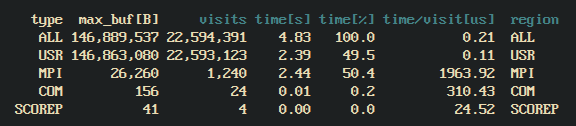
\includegraphics[width=1\linewidth]{./img/scorep_128_100.png}
	\caption{Tracing result for problem size of 128x128. Most time (around 50\%) is spent in MPI as expected. }%
	\label{fig:./img/scorep_128_100}
\end{figure}

\begin{figure}[htpb]
	\centering
	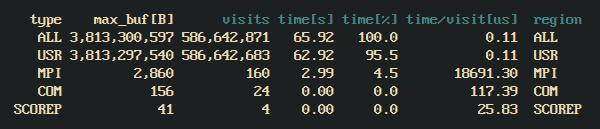
\includegraphics[width=1\linewidth]{./img/scorep_2048_10.png}
	\caption{Using a larger problem size of 2048x2048 MPI time becomes almost negligible (around 4\%)}%
	\label{fig:./img/scorep_2048_10}
\end{figure}
For large problems the number of iterations does not seem to change the result too much.

Looking at user time we can also see that most of the time is spent accessing vector items:
\begin{figure}[htpb]
	\centering
	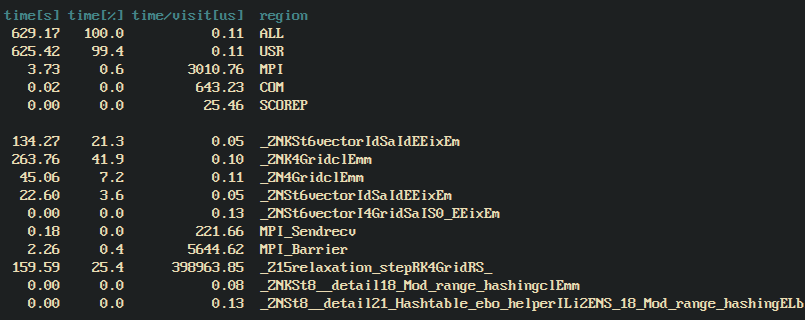
\includegraphics[width=1\linewidth]{./img/scorep_funcs.png}
	\caption{We can see that 25\% of time is spent \texttt{relaxation\_step()} doing actual computation. 42\% of the time is spent fetching elements from the grid}%
	\label{fig:/img/scorep_funcs}

\end{figure}
\subsubsection{Insights from tracing}
Using this information we could optimize memory access further (speed up index calculation).

\end{document}
